%%%%%%%%%%%%%%%% Springer %%%%%%%%%%%%%%%%%%%%%%%%%%%%%%%%%%


% RECOMMENDED %%%%%%%%%%%%%%%%%%%%%%%%%%%%%%%%%%%%%%%%%%%%%%%%%%%
\documentclass[graybox]{svmult}

% choose options for [] as required from the list
% in the Reference Guide

\usepackage{mathptmx}       % selects Times Roman as basic font
\usepackage{helvet}         % selects Helvetica as sans-serif font
\usepackage{courier}        % selects Courier as typewriter font
\usepackage{type1cm}        % activate if the above 3 fonts are
                            % not available on your system
%
\usepackage{makeidx}         % allows index generation
\usepackage{graphicx}        % standard LaTeX graphics tool
                             % when including figure files
\usepackage{multicol}        % used for the two-column index
\usepackage[bottom]{footmisc}% places footnotes at page bottom

% see the list of further useful packages
% in the Reference Guide
\usepackage{url}
\usepackage{array}

\usepackage[utf8]{inputenc} % please use UTF8 encoding

%\usepackage[round]{natbib} % if spbasic is used

\makeindex             % used for the subject index
                       % please use the style svind.ist with
                       % your makeindex program

%%%%%%%%%%%%%%%%%%%%%%%%%%%%%%%%%%%%%%%%%%%%%%%%%%%%%%%%%%%%%%%%%%%%%%%%%%%%%%%%%%%%%%%%%

\begin{document}

\title*{Using \emph{lemonUby} 
for data integration on the Multilingual Semantic Web}
 \titlerunning{Using \emph{lemonUby} 
for multilingual data integration} 
\author{Judith Eckle-Kohler, Iryna Gurevych, John McCrae and Christian Chiarcos}
% Use \authorrunning{Short Title} for an abbreviated version of
% your contribution title if the original one is too long
\institute{
Judith Eckle-Kohler \at Ubiquitous Knowledge Processing Lab  (UKP-TUDA),  
Technische Universit{\"a}t Darmstadt, Germany, \url{www.ukp.tu-darmstadt.de}
\and
Iryna Gurevych \at Ubiquitous Knowledge Processing Lab  (UKP-TUDA),  Technische Universit{\"a}t Darmstadt and
Ubiquitous Knowledge Processing Lab (UKP-DIPF),
German Institute for Educational Research and Educational Information, Germany, \url{www.ukp.tu-darmstadt.de},
\and
John McCrae \at CITEC, Universit{\"a}t Bielefeld, Germany, \url{jmccrae@cit-ec.uni-bielefeld.de}
\and
Christian Chiarcos \at  Information Sciences Institute, University of Southern California, USA, \url{chiarcos@isi.edu}
 }

%
% Use the package "url.sty" to avoid
% problems with special characters
% used in your e-mail or web address
%
\maketitle

\abstract*{Each chapter should be preceded by an abstract (10--15 lines long) that summarizes the content. The abstract will appear \textit{online} at \url{www.SpringerLink.com} and be available with unrestricted access. This allows unregistered users to read the abstract as a teaser for the complete chapter. As a general rule the abstracts will not appear in the printed version of your book unless it is the style of your particular book or that of the series to which your book belongs.
Please use the 'starred' version of the new Springer \texttt{abstract} command for typesetting the text of the online abstracts (cf. source file of this chapter template \texttt{abstract}) and include them with the source files of your manuscript. Use the plain \texttt{abstract} command if the abstract is also to appear in the printed version of the book.}

\abstract{
This chapter addresses lexicon-based methods for data integration on the Multilingual Semantic Web.
It presents use cases of  a new lexical resource integrated in the Semantic Web called 
\emph{lemonUby} which combines data from the standardized lexical resource UBY with the principled model, \emph{lemon},
for representing lexical data on the Web. This resource provides not only 
rich information about many lexical entries in two languages, it is also
significantly linked both within its component resources and to other
lexical resources and terminology repositories on the Web. 
This chapter describes further linkings of \emph{lemonUby}, such as 
the linking with the MASC corpus. 
A particular focus are methods for cross-lingual linking of verb senses
on the fly. We present results for the
cross-lingual linking of the English VerbNet and two German lexica rich in verbs.
}

%\emph{lemonUby} contains the English WordNet, FrameNet, VerbNet, Wiktionary and OmegaWiki, and German Wiktionary and OmegaWiki. 
%It describes models and terminology repositories for lexical resources and
%introduces methods for  multilingual data integration which are based on these.



\section{Motivation}

Lexical resources in the multilingual Linked Open Data cloud play an
important role for the development of the Multilingual Semantic Web,
because they can be used for cross-lingual linking and localization of Web
content. While many lexical resources, especially terminological resources, are
already available on the Web, syntactic descriptions, in particular of verbs, are largely
missing so far.
In the context of lexicalizing relational knowledge (such as, e.g.,
$like(Experiencer;Theme)$) in multiple languages, resources providing
fine-grained syntactic information on verbs are required on a large scale
and for many languages. Verbs are often used to express relations, e.g.
the relation $like(Experiencer, Theme)$ can be lexicalized syntactically as $NP~likes~NP$.

\section{Approaches to data integration}
Recently, the language resource community has begun to explore the opportunities offered by the Semantic
Web, lead by the formation of the Linguistic Linked Open Data (LLOD) cloud
and an increasing interest in making use of Linked Open Data principles in the context
of Natural Language Processing (NLP) and Linguistics  \cite{chiarcos2012linked}. 
The use of RDF supports data integration and offers a large body of tools for accessing this data.
Furthermore, the linked data approach gives rise to novel research questions in the context of
language resources and their application.


 For lexical resources, data integration has been in
 the focus of interest for many years, resulting in numerous mappings and linkings of lexica, as well as 
standards for representing lexical resources, such as the ISO 24613:2008 Lexical Markup Framework
(LMF) \cite{francopoulo2006lexical}. In this context, the LLOD cloud can be considered as a new data integration platform, enabling linkings not only between lexical resources, but also between lexical resources and
other language resources, such as terminology resources and corpora.

%Many lexical resources have already been included in the LLOD cloud, e.g., WordNet, Wikipedia 
%(DBpedia \cite{Bizer_Lehmann_Kobilarov_Auer_Becker_Cyganiak_Hellmann_2009}),
%and Wiktionary, as well as integrated resources, such as an integrated version of WordNet and Wiktionary\cite{mccrae2012integrating}, or of  WordNet and Wikipedia (BabelNet, \cite{navigli2012babelnet}).
%There has also been some work towards the integration of FrameNet \cite{baker1998berkley} to the Semantic Web \cite{narayanan2003framenet}.
%All these resources provide a substantial body of lexical knowledge, including semantic relations, multilingual
%information and encyclopedic knowledge.

%However, what is missing in the LLOD cloud is a large-scale lexical resource rich in lexical information on
%verbs, including aspects such as syntactic behaviour and how semantic arguments
%of verbs can be realised
%syntactically. Such information is crucial for lexicalizing relational knowledge
%which is often expressed
%by using verbs, e.g., the relation $like(Experiencer, Theme)$ can be lexicalized syntactically as "NP likes NP".
%Such information is crucial for lexicalizing relational knowledge which is typically expressed
%by using verbs along with specific arguments.

\emph{lemon}, a lexicon model for representing and sharing ontology lexica, 
has been proposed as a common interchange format for lexical resources on the Semantic Web\cite{mccrae2012interchanging}. 
Making use of a common interchange format
is important, to integrate resources such as FrameNet and WordNet, which have
been characterised as
complementary resources~\cite{baker2009wordnet}. The RDF version of FrameNet currently available does not adhere to an interchange format such as \emph{lemon}, but is specific to the underlying data model of FrameNet.

%In the current LLOD cloud, large-scale lexical resources rich in encyclopedic knowledge, such as DBPedia, are 
%predominant, while
%the size and diversity of lexical resources rich in linguistic knowledge, particularly for verbs,
% is limited so far.
% There has already been some work towards the integration of FrameNet \cite{baker1998berkley} to the Semantic Web \cite{narayanan2003framenet},
%as well as WordNet 
%\cite{van2006conversion}, WordNet and Wiktionary\cite{mccrae2012integrating}, and recently BabelNet as a multilingual
%lexical resource integrating WordNet and Wikipedia \cite{navigli2012babelnet}.
% In the Semantic Web, several versions of WordNet REF
%and FrameNet REF have been available as linked data for quite same time, but due to the LLOD movement
%new resources such as
%Wiktionary REF and BabelNet REF have been added just recently.
%However, the LLOD cloud contains no large-scale lexical resource yet, which is rich in lexical information on
%verbs, including aspects such as their syntactic behavior and how semantic arguments of verbs can be realized
%syntactically. Such information is crucial for lexicalizing relational knowledge which is typically expressed
%by using verbs along with specific arguments.

Independently from linked data principles and Semantic Web technology, the large-scale lexical-semantic resource UBY \cite{gurevych2012uby} has been developed.\footnote{\url{http://www.ukp.tu-darmstadt.de/uby/}}
UBY is based on LMF and has currently integrated 10 lexical resources
 in English and German. A subset of these resources
is interlinked at the word sense level. 

Recently, a selection of UBY lexica have been converted to
the \emph{lemon} format, resulting in the large resource \emph{lemonUby}.
This resource
%The data-set presented in this paper, \emph{lemonUby}, is the result of
%converting a selection of UBY lexica to
%the \emph{lemon} format:
%it 
contains interoperable and interlinked versions of WordNet \cite{Fellbaum1998}, FrameNet \cite{baker1998berkley},
VerbNet \cite{kipper2008large}, English and German Wiktionary\footnote{\url{http://www.wiktionary.org}},
 and the English and German entries of
OmegaWiki.\footnote{\url{http://www.omegawiki.org}}
\emph{lemonUby} has been linked to other lexical resources (e.g. the WordNet versions 2.0 and 3.0 in the LLOD)
 and to terminology resources in the LLOD cloud.
The linking to terminology resources comprises a linking of linguistic terminology used in
\emph{lemonUby}  to 
ISOCat\footnote{\url{http://www.isocat.org/}}, the implementation of the ISO 12620:2009 Data Category Registry, as well as a linking to
the Ontologies of Linguistic Annotation (OLiA,\cite{chiarcos2008ontology,chiarcos2012ontologies}).

%OLiA represents a repository of annotation
%terminology that act as a central reference hub for 
%linguistic annotations in about 70 languages, for which they provide formal definitions of annotation
%schemes for various linguistic phenomena as OWL/DL ontologies. Further, OLiA establishes interoperability between
%different annotation schemes by linking them to an overarching `Reference Model'.
%Through the OLiA Reference Model, interoperability with community-maintained data
%category registries can be achieved, as it is linked to both the
%General Ontology of Linguistic Description \cite[GOLD]{farrar2003markup}
%(GOLD) and ISOCat.
%
%The OLiA ontologies (and the terminology repositories it is linked with) can be used to represent, compare and integrate linguistic annotations in corpora on the basis of formal concepts rather than arbitrary strings \cite{chiarcos2010towards}, and in this function, they also enjoy a certain popularity in NLP applications \cite{hellmann2012nif}. In a Linked Data context, they explicitly allow to compare the linguistic categories used in \emph{lemonUby} with the morphosyntactic annotations in linguistic corpora, if these are represented in RDF. 
% 

% To summarize, our contributions are threefold: (i) an interlinked lexical resource rich
%in linguistic information on verbs, %also containing a lot of multilingual information, 
%(ii) a mapping of the lexicon model UBY-LMF to \emph{lemon}, and (iii)
%the linking of \emph{lemonUby} to other language resources in the LLOD cloud.

%Moreover, the
%format chosen for the RDF versions of FrameNet and WordNet 
% was specific to the underlying data model of these two resources which have been characterized as
%complementary by \cite{Baker:2009}. 
%However, the LLOD cloud contains no large-scale lexical resource yet which is rich in lexical information on
%verbs, including aspects such as their syntactic behavior and how semantic arguments of verbs can be realized
%syntactically. Such information is crucial for lexicalizing relational knowledge which is typically expressed
%by using verbs along with specific arguments.
%The dataset \emph{lemonUby} which we present in this paper addresses these gaps: 
%it contains interoperable and interlinked versions of WordNet [FEL 98], FrameNet [BAK 98],
%VerbNet [KIP 08], and multilingual OmegaWiki (www.omegawiki.org). 
%\emph{lemonUby} is linked to the LLOD cloud and has a number of 
%additional features that add significant value to the LLOD cloud. We will describe these features and the creation
%of this dataset in the following sections.

% \section{An interchange format for lexical resources on the Semantic Web: \emph{Lemon}}

\begin{figure}
 \begin{center}

 	 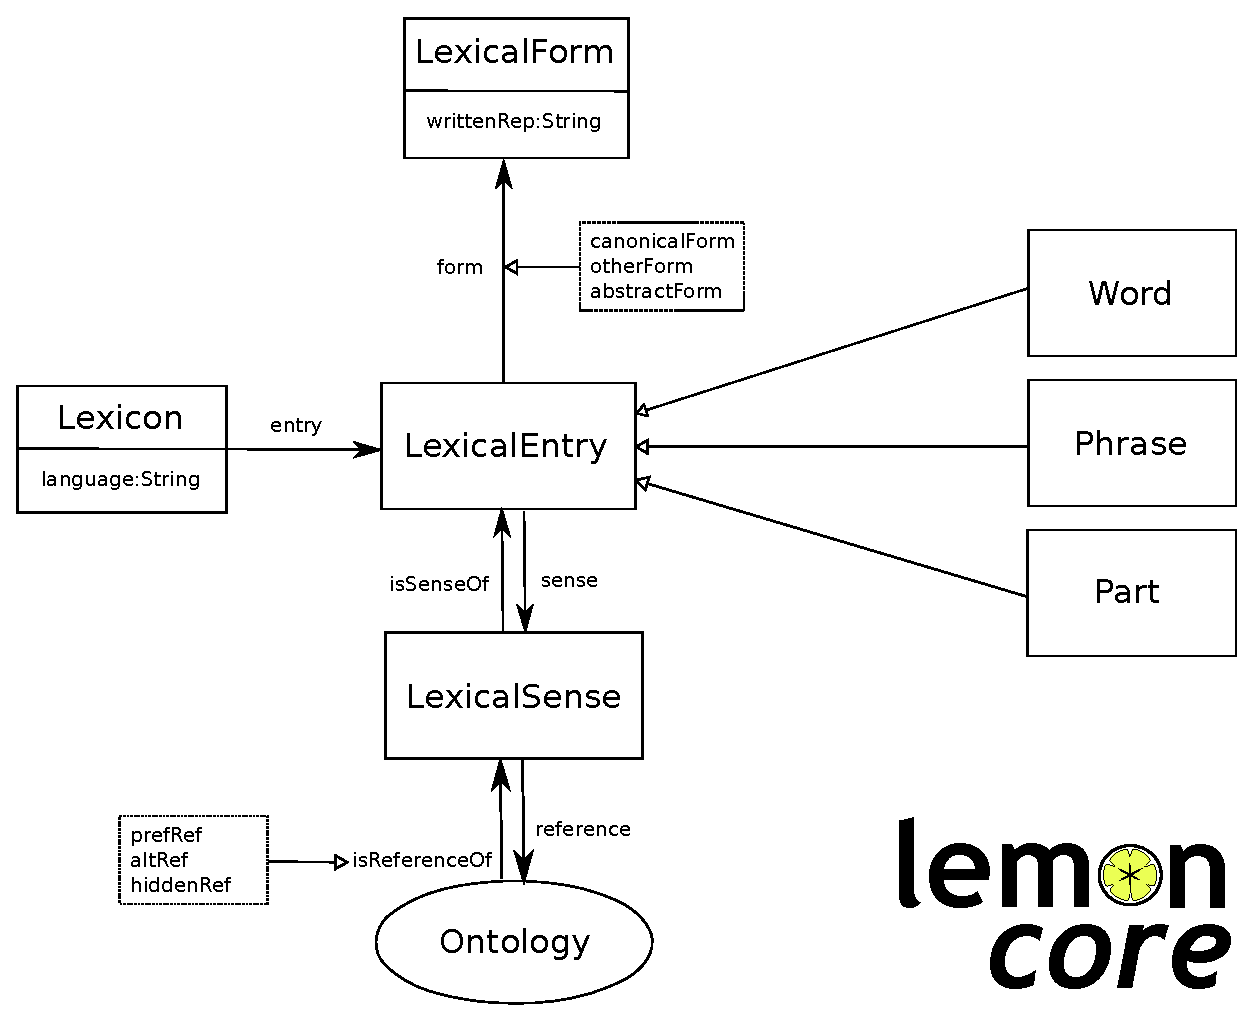
\includegraphics[width=1.0\columnwidth]{images/lemon-core}

 \end{center}
\caption{The core of the \emph{lemon} model\label{lemon-core}}
\end{figure}

\emph{lemon}, a lexicon model for representing and sharing ontology lexica, 
has been proposed as a common interchange format for lexical resources on the Semantic Web\cite{mccrae2012interchanging}. 
Making use of a common interchange format
is important, to integrate resources such as FrameNet and WordNet, which have
been characterised as
complementary resources~\cite{baker2009wordnet}. The RDF version of FrameNet currently available does not adhere to an interchange format such as \emph{lemon}, but is specific to the underlying data model of FrameNet.

%There has been significant work towards integrating lexical resources using RDF and 
%Semantic Web principles~\cite{chiarcos2011towards}, and many resources have already
%been converted to RDF,  notably the conversion of WordNet 
%\cite{van2006conversion}. They provided a simple mapping from WordNet to RDF, and 
%augmented it with OWL semantics so that reasoning could be applied to the structure of the resource.
%However, the format chosen for this resource was specific to the underlying data model of WordNet. 
For this reason, the \emph{lemon} model\cite{mccrae2012interchanging} was proposed  that supports publishing 
lexical-semantic resources as linked data on the basis of the following principles:

\begin{description} 
\item[LMF-based]: To allow easy conversion from non-linked data resources.
\item[RDF-native]: Publishing as linked data, with RDFS and OWL used to describe
  the semantics of the model.
\item[Modular]: Separation of lexicon and ontology layers, so that \emph{lemon} lexica can be linked to existing ontologies
in the linked data cloud.
\item[Externally defined data categories]: Linking to data categories in
  annotation terminology repositories, rather than being limited to a specific part-of-speech tag set.
\item[Principle of least power]: The smaller the model and the less expressive the language, 
	the wider its adoption and the higher the reusability of the
	data\cite{shadbolt2006semantic}.
\end{description}

This core model 
is illustrated in Fig.\ \ref{lemon-core}, which 
defines the
basic elements used by all lexica published as linked data. In addition to this there
are a number of modules used to model linguistic description, syntax, morphology 
and relationships between lexica~\footnote{More detail of the model and descriptions of
the modules can be found at \url{http://lemon-model.net}}.

%\emph{lemon} has been used as a basis for integrating the data of the 
%English Wiktionary, a (human-readable) 
%dictionary created along `wiki' principles, with  
%the RDF version of WordNet \cite{mccrae2012integrating}. \emph{lemon}'s similarity
%to the WordNet model made this conversion straight-forward, with only the need for
%a slight change in modelling to accommodate inflectional variants of lexical
%entries.


 \section{\emph{lemon} and UBY-LMF}
\begin{figure}
 \begin{center}

 	 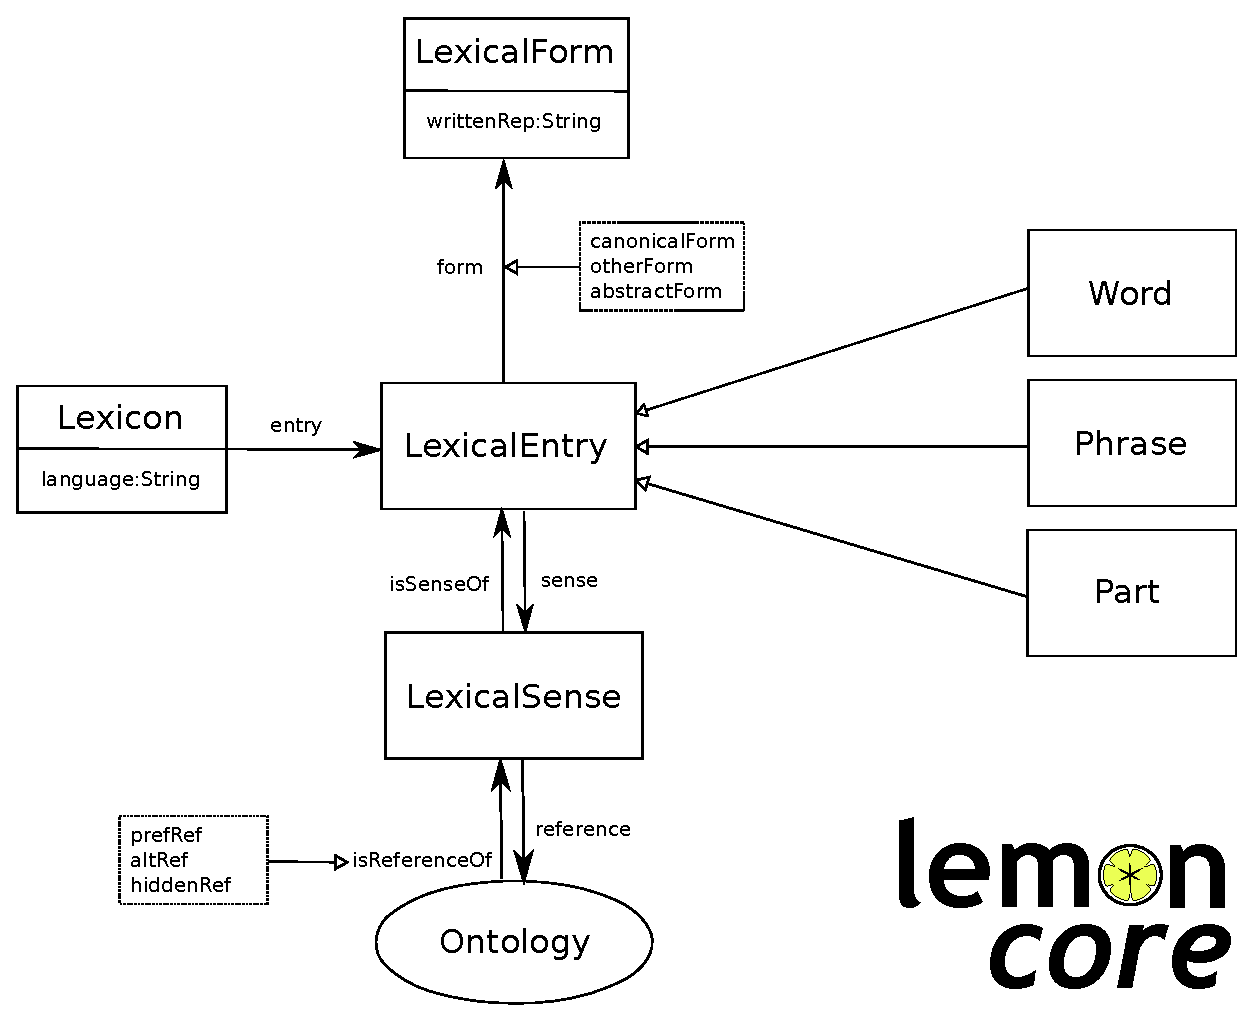
\includegraphics[width=1.0\columnwidth]{images/lemon-core}

 \end{center}
\caption{The core of the \emph{lemon} model\label{lemon-core}}
\end{figure}

The \emph{lemon} model\cite{mccrae2012interchanging} is a  lexicon model for representing and sharing ontology lexica.
It supports publishing 
lexical-semantic resources as linked data on the basis of the following principles:

\begin{description} 
\item[LMF-based:]{To allow easy conversion from non-linked data resources.}
\item[RDF-native:]{Publishing as linked data, with RDFS and OWL used to describe
  the semantics of the model.}
\item[Modular:]{Separation of lexicon and ontology layers, so that \emph{lemon} lexica can be linked to existing ontologies
in the linked data cloud.}
\item[Externally defined data categories:]{Linking to data categories in
  annotation terminology repositories, rather than being limited to a specific part-of-speech tag set.}
\item[Principle of least power:]{The smaller the model and the less expressive the language, 
	the wider its adoption and the higher the reusability of the
	data\cite{shadbolt2006semantic}.}
\end{description}

This \emph{lemon} core model is illustrated in Fig.\ \ref{lemon-core}, which defines the
basic elements used by all lexica published as linked data. In addition to this, there
are a number of modules used to model linguistic description, syntax, morphology 
and relationships between lexica.\footnote{More details on the model and descriptions of
the modules can be found at \url{http://lemon-model.net}}

%UBY is both a network of interlinked lexical-semantic resources 
%and a project on continuous integration and linking of lexical resources for NLP applications.
% It is motivated by the
%observation that an essential requirement in NLP is the availability of a wide range of lexical resources that can be used for many different NLP tasks. In a continuous process, such resources
%are integrated into UBY by means of (i) making them inter-operable  and (ii)
%linking them to other resources in UBY at the sense level.

%UBY has currently integrated 10 LRs in two languages, see www.ukp.tu-darmstadt.de/uby. Only 8 of these LRs have open licenses and 
%can be offered as a UBY database dump for download: English WordNet, Wiktionary, Wikipedia, FrameNet and VerbNet, German Wikipedia, Wiktionary, and multilingual OmegaWiki. 
%A subset of these LRs is linked at the word sense level and these sense alignments are open as well. 
%There are monolingual sense alignments between VerbNet--FrameNet\footnote{\url{http://verbs.colorado.edu/semlink/}} and 
%VerbNet--WordNet\footnote{\url{http://verbs.colorado.edu/~mpalmer/projects/verbnet}} as well as between WordNet--Wikipedia \cite{niemann2011peoples} and WordNet--Wiktionary  \cite{meyer2011what}. In addition, Uby provides cross-lingual sense alignments between WordNet and the German OmegaWiki \cite{gurevych2012uby}, also including the inter-language links already given in Wikipedia and OmegaWiki.
%
%UBY databases can be created according to specific application needs: a user might want to use only a subset of the LRs integrated into UBY, convert them to UBY-LMF and import them into
%a database. Any UBY database can be accessed with a single Java-API which is continuously developed along with the conversion tools in an Open Source Project on Google Code (code.google.com/p/uby).
%UBY and UBY-LMF are CC-licensed and the UBY-related software is licensed under the open Apache license. 

In UBY, interoperability is achieved by standardizing lexical resources according to UBY-LMF \cite{ecklekohler2012uby,TUD-CS-2013-0003}, a lexicon
model which is a full-fledged instantiation of the ISO standard LMF, specifically for NLP.
%instantiates the Lexical Markup Framework (LMF, ISO 24613:2008, \cite{francopoulo2006lexical}). 

In comparison to the \emph{lemon} lexicon model,  UBY-LMF is similar in two aspects: first it is LMF-based, and second,
it uses externally defined data categories from
ISOCat.\footnote{\url{http://www.isocat.org/rest/dcs/484}}
In contrast to \emph{lemon}, however, UBY-LMF is based on two quite different principles:
\begin{description} 
\item[Principle of Adoption:]{UBY-LMF has been designed to fully cover a wide range of heterogeneous lexical resources
without information loss.}
%This resulted  in a fine-grained model of lexical information types, which ranges from morphology and lexical syntax to lexical semantics and the mapping between syntactic and semantic arguments. 
\item[Independence of implementation:]{UBY-LMF  is independent of any particular implementation. There are many ways to implement an LMF lexicon model \cite{francopoulo2007lexical}, including RDF.} 
\end{description}


%UBY-LMF, is currently represented in two ways: first, as a DTD, and second, as a Java Object-Relational Mapping by means of the Hibernate framework\footnote{\url{http://www.hibernate.org}}, 
%which allows mapping any instance of UBY-LMF either to a SQL database or to an XML file.
%Both ways of representing UBY-LMF do not require the use of globally unique identifiers (URIs). 
%However, an implementation of UBY-LMF in RDF would be possible as well.
%, since UBY-LMF as such is independent of any particular implementation or 
%serialization and an LMF lexicon model can be implemented in many ways \cite{francopoulo2007lexical}.

% JEK I would not call it extension
%An extension of LMF to include URIs \cite{Francopoulo2007}, and full-fledged RDF linearizations of LMF have been suggested, e.g., in the context of the Lexicon Model for Ontologies (Lemon) as described by McCrae et al. (2011)\nocite{McCrae2011}.
%An implementation of LMF to include URIs has already been suggested\cite{francopoulo2007lexical}.
%In fact, providing lexical resources, in particular interlinked resources such as UBY, as linked data is a very natural
%step to take and
%allows us to integrate UBY-LMF-based resources with other resources previously converted to RDF. 
%e.g., in the context of the developing Semantic Web.

%, and full-fledged RDF linearizations of LMF have been suggested, e.g., 
%in the context of the Lexicon Model for Ontologies (Lemon) for a variant of LMF as described by McCrae et al. (2011)\nocite{mccrae2011linking}.
We performed a
mapping of UBY-LMF to \emph{lemon} which allows conversion of lexical resources in UBY-LMF format to \emph{lemon} format.
%Apart from the fact that the mapping of UBY-LMF to \emph{lemon} is an interesting task per se, because \emph{lemon} links lexical resources and 
%ontologies, there is another reason for this mapping. 
%The LMF standard is not an open standard (in the sense that its specification is not freely available), while \emph{lemon} provides an
%interchange format which fully complies with open data and open access principles.

%An extension of LMF to include URIs \cite{Francopoulo2007}, and full-fledged RDF linearizations of LMF have been suggested, e.g., in the context of the Lexicon Model for Ontologies (Lemon) as described by McCrae et al. (2011)\nocite{McCrae2011}.

%Originally, Uby was implemented using the Lexical Markup Framework, a standard aiming for interoperability among lexical-semantic resources.

% LMF is no format, it is an abstract standard
%First, the LMF standard is not an open standard (in the sense that its specification is not freely available), and,
% according to the experience of UBY, the application of the standard requires % making 
%NLP domain-specific modifications to the abstract model defined by the standard.
%Second, the currently used implementation of UBY-LMF does not consider how resources can be uniquely identified on the web. 


%and in its frequently used
% LMF does not say anything about serialization, XML is just an illustrative example
 %serialization as XML, it does not consider how resources can be uniquely identified on the web. 
%Furthermore, according to the experience of UBY, application of the standard requires % making 
%NLP domain-specific modifications to the standard schema.

%An RDF formalization tackles %of LMF allows us to tackle 
%some of these problems, and this has been suggested by the LMF developers themselves% \citep{francopoulo2009multilingual}
%.\footnote{\url{http://www.tagmatica.fr/lmf/LMF_revision_14_In_OWL29october2007.xml}}

%LMF is grounded in earlier research on feature structures (i.e., directed acyclic graphs) that have been suggested as a generalization over resource-specific data structures \citep{veronis-ide92-feature-structures-for-lexical-dbs}.
%Feature structures are a flexible and general formalism, which became the basis for subsequent standardization, in particular, in LMF.
%\citealp{francopoulo2006lexical}).

% LMF represents a metamodel % aiming to provide a standard 
% to represent semantic information in NLP lexicons and machine-readable dictionaries.
% It has been successfully applied to develop resources, including the different Uby data sets.

%Converting a lexical resource in UBY-LMF format to lemon requires a mapping of the UBY-LMF lexicon model to the lemon lexicon model. 

Although both UBY-LMF and \emph{lemon} are based on LMF, the mapping revealed substantial differences. These are mainly due to the fact that 
\emph{lemon} is a model for ontology lexica where the lexicon and ontology layers are kept separate. Thus, sense representations in \emph{lemon} primarily consist of references to the associated ontology
where a rich and domain-specific sense definition is provided. 
The development of UBY-LMF, on the other hand, has been driven by the requirement to cover a large variety of
 lexical information types, which ranges from morphology and lexical syntax to lexical semantics and the mapping between syntactic and semantic arguments. 
Thus, the resulting lexicon model makes use of very fine-grained sense specifications which are often grounded in linguistic theories.
%e.g. Frame Semantics (the basis of FrameNet) or the Levin alternation classes of verbs \cite{levin93} (the basis of VerbNet).


 % UBY-LMF, UBY, mapping of UBY-LMF to lemon
 %\section{Comparison of  \emph{lemon} and UBY-LMF}
%\begin{verbatim}
%- modeling issues: argument mapping to capture syntactic behavior -> JEK&JM
%- usage/register information represented differently
%- lemonUBYlite: where, which license
%\end{verbatim}
%The actual conversion  of UBY lexica to \emph{lemon} was achieved by means of
%an XML style sheet transform~\footnote{The XSL file can be downloaded at
%\url{https://raw.github.com/jmccrae/lemon.api/master/src/main/resources/xslt/ubylmf2lemon.xsl}}.
%The following UBY lexica were converted: WordNet, FrameNet, VerbNet, English and German Wiktionary, and the English and German entries of OmegaWiki. 
%Pairs of these resources are linked at the sense level:
%there are monolingual links between 
%VerbNet--FrameNet\footnote{\url{http://verbs.colorado.edu/semlink/}}, 
%VerbNet--WordNet\footnote{\url{http://verbs.colorado.edu/~mpalmer/projects/verbnet}},
%WordNet--FrameNet \cite{tonelli-pighin:2009:CoNLL,laparra-rigau:2009:RANLP09}, as well as between WordNet--Wiktionary  \cite{meyer2011what}. Moreover, \emph{lemonUby} provides cross-lingual links between WordNet and the German Ome\-ga\-Wiki \cite{gurevych2012uby}, also including the inter-language links already given in OmegaWiki.

%The resulting resource 
%\emph{lemonUby} has been published at
%\url{http://lemon-model.net/lexica/uby}
%and is available under an open CC-BY-SA license. 
%The choice of a share-alike
%license was due to UBY being published under the same license. Statistics for
%the resources are given in table \ref{triples}\footnote{At the time of
%submission, en.wiktionary.org resource was not available, we expect to have
%this ready in time for final publication}.
%Based on the mapping of UBY-LMF to lemon, we performed a conversion of the following
%LRs which demonstrate the main parts of a UBY-LMF -- lemon
%mapping: WordNet, FrameNet, VerbNet, and multilingual OmegaWiki. 
%These LRs illustrate a number of differences between the two lexicon models in a 
%prototypical way. First, we will describe differences in the representation of senses, 
%then we will summarize more general differences that
%had to be harmonized via a mapping. The actual mapping was achieved by means of
%an XML stylesheet transform~\footnote{The XSL file can be downloaded at
%\url{https://raw.github.com/jmccrae/lemon.api/master/src/main/resources/xslt/ubylmf2lemon.xsl}}.

\emph{lemonUby} nicely illustrates how the two lexicon models represent senses in different ways:
\begin{itemize}
\item In line with previous authors~\cite{mccrae2012integrating}, synsets in
  WordNet and OmegaWiki are considered as ontology classes. Hypernym
  relationships stated in the lexicon are mapped directly to subclass
  relationships in the ontology. In UBY-LMF, Synset is part of the lexicon.
%\item Synsets, which are used in WordNet and OmegaWiki, are considered as
%  entryless senses in \emph{lemon}. Previous
%  conversions~\cite{mccrae2012integrating} have treated synsets as ontological
%  classes, however here the 
\item The semantic predicate in UBY-LMF is used to represent semantic frames from 
  FrameNet \cite{TUD-CS-2013-0003}; frames consist of senses which evoke the same situation with participants. 
  Thus, senses in the same semantic frame are semantically related, but not synonymous; 
  e.g., the verbs {\em love} and {\em hate} are both in the same frame. %Experiencer subj frame
In \emph{lemon} a 
{\em broader sense} is used to capture semantic predicates.
\item VerbNet verb classes and their hierarchical organization correspond to  
  subcat[egorization] frame set in UBY-LMF. VerbNet classes group verbs that
share the same syntactic subcategorization frame, semantic roles, selectional
restrictions, and semantic predicate. Although the resulting verb classes are
semantically coherent, the semantic relatedness of verb senses in a VerbNet class is much more
distant that in FrameNet, e.g., the verbs {\em believe}, {\em swear} and {\em doubt} are in the same class.
%conjecture-29.5-1.
%semantically related and 
%  syntactically similar senses; the semantic relatedness of senses in one VerbNet class is much more
%distant that in FrameNet. 
Verb classes in \emph{lemon} are represented by a broader sense as well.
The hierarchic organisation of VerbNet classes is thus lost, but this can be
reconstructed by means of an axiomatic description of subcategorization frames in
order to create a hierarchy similar as in the LexInfo linguistic
ontology~\cite{mccrae2011linking}.
\item Syntactic behaviour in UBY-LMF mainly provides information on
subcategorization frames, which are specified by means of syntactic arguments
with rich morpho-syntactic information attached
\cite{TUD-CS-2012-0024}.
SyntacticBehaviour is merely a property instead of a node in \emph{lemon}: in 
contrast to LMF, there is no need for an explicit link between senses and
subcategorization frames. Instead this information  can be 
reconstructed from the \emph{synArg} - \emph{semArg} mapping.
Lexica which do not specify semantic arguments, e.g., GermaNet \cite{Kunze02},
must provide a specific annotation to allow this information to be represeneted.
\item Translations are represented differently. UBY-LMF uses Equivalent for 
  translations that are not sense-disambiguated \cite{TC32012}, where as
  \emph{lemon} requires that this link is made at the sense level. In the case
  where it was not possible to infer the sense, the lexical entries a `stub'
  lexical entry with a single sense.\footnote{UBY-LMF can also represent sense-disambiguated 
    translations by means of a sense axis which connects senses from different
  lexica.}
\end{itemize}
%To sum up, 
Most of the differences between UBY-LMF and \emph{lemon} derive from the fact that 
\emph{lemon} keeps the lexicon and ontology layers separate. In this way, sense representations in
\emph{lemon} are more compact compared to the more distributed sense representations in UBY-LMF.

%the separation of  the principal distinction between UBY-LMF and \emph{lemon}the separation of 
%a principal difference between UBY-LMF and \emph{lemon} is redundant vs. compact  representation of information.
%For instance, the synset class is merged into the lemon:LexicalSense, while UBY might provide information on
%synonyms by sense relations of type synonym and by the Synset class (which groups synonymous senses).
%Since UBY-LMF is populated fully-automatically, the consistency of redundant information can be ensured.
%An example is SyntacticBehaviour which is not used in \emph{lemon}: while the information to which sense a subcat frame belongs to, can be reconstructed from the \emph{synArg} - \emph{semArg} Mapping, the 
%relationship between sense and syntactic behaviour can not be recovered for LR which do not specify
%semantic arguments, e.g., GermaNet.

%\begin{table}
%  \begin{tabular}{|p{3cm}|c|}
%    \hline
%    Resource & Triples \\
%    \hline
%    WordNet & 5,102,744 \\
%    VerbNet & 570,256 \\
%    FrameNet & 1,110,763 \\
%    OmegaWiki English & 6,173,515 \\
%    OmegaWiki German & 5,310,551 \\
%    Wiktionary German & 4,766,917 \\
%    \hline
%    Total & 23,034,746 \\
%    \hline
%  \end{tabular}
%  \caption{Number of triples for each resource\label{triples}}
%\end{table}
    
 %conversion of UBY resources to lemon
 %\section{Linking \emph{lemonUby} to lexical-semantic resources}

As UBY is derived from existing resources the simplest links to create are those
to other RDF versions of the resources that compose UBY. For WordNet these links 
are simply created by mapping the data of UBY to the linked data version of 
WordNet 3.0~\footnote{\url{http://semanticweb.cs.vu.nl/lod/wn30/}}. Here,
we provided links at both the sense level and at the lexical entry level 
(lexical entries are ``words'' in WordNet 3.0). We found that this worked apart
from 7 senses that did not map, which we believe is due to a bug in the 
WordNet API. 

In addition, we provided links to two existing resources that are also widely
used, firstly to RDF WordNet 2.0~\cite{van2006conversion}. As the sense identifiers are
different to the WordNet version used by UBY we only attempted to link at the lexical 
entry level, using the assumption that the lemmas were the same. Secondly, we 
linked to the RDF export of Wiktionary~\footnote{\url{http://wiktionary.dbpedia.org}}.
For this resource, we first linked the WordNet data on the lexical entry level using 
the lemma and part-of-speech information. This was mostly effective, however some
elements were initially missing due to category misalignment (Wiktionary has
``Initialism'' as a part-of-speech, for example for ``IBM'', whereas WordNet
counts these as nouns); we added manual corrections to compensate 
for this. Statistics for all mappings are given in table \ref{mapping-stats}.

\begin{table}
  \begin{tabular}{|l|l|p{3cm}|}
    \hline
    Uby Resource & Other Resource & Links (Percentage of Uby resource) \\
    \hline
    WordNet & WordNet 3.0 & 206,773 (99.9\%)\\
    WordNet & WordNet 2.0 & 84,416 (40.8\%) \\
    WordNet & Wiktionary & 76,294 (36.9\%) \\
    \hline
  \end{tabular}
  \caption{Number of external links created between lemonUby and other resources
  in the LLOD cloud \label{mapping-stats}}
\end{table}
  	  
  






 
\section{Linking \emph{lemonUby} with corpora} % the latter is an outlook, but mentioned as such


%Within the LLOD cloud, the Ontologies of Linguistic Annotation (OLiA,\cite{chiarcos2008ontology,chiarcos2012ontologies})
% represent a repository of annotation
%terminology that act as a central reference hub for 
%linguistic annotations in about 70 languages, for which they provide formal definitions of annotation
%schemes for various linguistic phenomena as OWL/DL ontologies. Further, OLiA establishes interoperability between
%different annotation schemes by linking them to an overarching `Reference Model'.
%Through the OLiA Reference Model, interoperability with community-maintained data
%category registries can be achieved, as it is linked to both GOLD and ISOCat.
%Unlike these \emph{evolving} repositories that aim for definitions and categories that are generally applicable, the OLiA Reference Model only serves as an aggregation point for the annotation schemes directly linked to it. It generalizes over these schemes, interprets them against other terminology repositories, and thereby provides a stable interface between linguistic annotations and these repositories in-the-making.


%An ontology-based approach allows to express complex relationships among reference categories and between reference categories and annotations. For the linking of Uby to the OLiA Reference Model, we created an ontology for the morphosyntactic concepts used in UBY-LMF, that redefined the enumeration of categories in the DTD was redefined with more elaborate hierarchical structures. This ontology is linked to the OLiA Reference Model by subClassOf relationships between its concepts and the Reference Model. As this linking is an \emph{interpretation}, it is physically separated in an independent `Linking Model', because different interpretations may be possible. 

The OLiA ontologies (and the terminology repositories it is linked with) 
%have been applied as a component of the \emph{lemon} model before \cite{mccrae2012interchanging}, and (as part of their original motivation), they 
can be used to represent, compare and integrate linguistic annotations in corpora on the basis of formal concepts rather than arbitrary strings \cite{chiarcos2010towards}.
% and in this function, they also enjoy a certain popularity in NLP applications \cite{hellmann2012nif}. 
In a Linked Data context, they explicitly allow to compare the linguistic categories used in \emph{lemonUby}
 with the morphosyntactic annotations in linguistic corpora, if these are represented in RDF. 
An RDF version of the MASC corpus \cite{ide-etal08-masc} has been produced,
%\footnote{
%    The current Linked Data version of the corpus, MASC 1.0.3, generated from data available under \url{http://datahub.io/dataset/masc}, is not yet linked with other resources as it will soon be deprecated by the release of a new version of the corpus and a revision of its data model.
%}
a resource that also provides FrameNet and WordNet annotations, and whose annotations can thus be directly compared with and combined with UBY resources.
We performed a linking of the FrameNet 1.5 version contained in \emph{lemonUby}
with the FrameNet annotations in the MASC corpus. As MASC provides FrameNet sense annotations
for different text genres and domains, this linking can be used to enrich FrameNet senses in
\emph{lemonUby} by genre and domain information. 

\section{Cross-lingual linking of verb senses}
The standardized format for English and German subcategorization frames defined in UBY-LMF can be exploited for the 
 linking of verb senses across English and German. We show in detail how such a linking based on
subcategorization frame information is performed on the fly and point out important properties of
the underlying representation of subcategorization frames related to this linking.
 
As an example, the cross-lingual linking of VerbNet and two German lexicons, i.e., the German wordnet GermaNet \cite{Kunze02} and the large syntactic subcategorization lexicon
IMSLex \cite{TUD-CS999-0006} is described and evaluated.
This is a particularly interesting linking, because it demonstrates how large lexica with a focus on particular information types in one language 
(e.g., syntactic subcategorization frames in IMSLex) can be enriched by complementary information from lexica in other languages (e.g., VerbNet). Both GermaNet and IMSLex contain detailed subcategorization information
for verbs, but they do not contain information on semantic roles
or selectional preferences for the arguments of verbs. Yet, they are the only large
German lexica\footnote{GermaNet provides information for 8626 verb lemmas, IMSLex for 10879 verb lemmas.} containing fine-grained subcategorization information which are freely available for research purposes.
%While GermaNet and IMSLex  both have an academic license, they are the only large scale 
%German lexicons containing detailed subcategorization information
% which are freely available for research purposes. However, they do not contain information on semantic roles
%or selectional preferences for the arguments of verbs. 
The cross-lingual linking
of these German lexicons and VerbNet provides access not only to information on semantic roles
or selectional preferences, but also to semantic role information from FrameNet via the VerbNet--FrameNet
linking in UBY.
%For a subset of the three lexicons, the results of the cross-lingual linking approach has been evaluated
%which yielded a precision of 72,68.

Finally, we compare the cross-lingual linking of verb senses using
 original UBY lexicons (based on UBY-LMF) with the linking of verb senses which is based on the
mapping of UBY-LMF to \emph{lemon}.



 
 \section{Conclusion}

This chapter describes methods for multilingual data integration on the Semantic Web which  rely 
crucially on semantically interoperable language resources, i.e., language resources which are linked to reference
terminology repositories, such as OLiA or ISOCat.
The use cases of \emph{lemonUby} described in this chapter give a good indication of the
potential benefits of linking language resources on the Web on a large scale.



\begin{acknowledgement}
The work on \emph{lemon} was developed in the context of the Monnet project, which is funded by the European Union FP7 program under
grant number 248458, the CITEC excellence initiative funded by the DFG (Deutsche Forschungsgemeinschaft).
The work on UBY has been supported by the Volks\-wagen Foundation as part of the Lichtenberg-Professorship Program under grant No.\ I/82806.
The research of Christian Chiarcos has been supported by the German Academic Exchange Service (DAAD) through a PostDoc fellowship at the University of Southern California.
We thank Silvana Hartmann, Michael Matuschek and Christian~M. Meyer for their contributions to this work.

\end{acknowledgement}

 \bibliographystyle{spbasic}
 %\bibliographystyle{spphys}
 \bibliography{bib}

\end{document}
